
%%%%%%%%%%%%%%%%%%%%%%%%%%%%%%%%%%%%%%%%%%%%%%%%%%%%%%%%%%%%%%%%%%%%%%%
%                            First Chapter                            %
%                         Problem Formulation                         %
%%%%%%%%%%%%%%%%%%%%%%%%%%%%%%%%%%%%%%%%%%%%%%%%%%%%%%%%%%%%%%%%%%%%%%%

\chapter{Posture Generation: Problem Formulation}
\label{cha:posture_generation_problem_formulation}

\nomenclature[z-PG]{PG}{Posture Generation}
\nomenclature[z-IK]{IK}{Inverse Kinematics}
\nomenclature[z-DoF]{DoF}{degrees of freedom}
\nomenclature[z-w.r.t]{w.r.t}{with respect to}
\nomenclature[x-I]{$\mathbb{I}_n$}{Matrix identity of dimension $n$}
\nomenclature[x-w]{$\wedge$}{cross product}
\nomenclature[a-F]{F}{a frame}
\nomenclature[a-W]{W}{the world frame}
\nomenclature[a-w]{w}{a wrench or a force}
\nomenclature[a-f]{f}{a force resultant}
\nomenclature[a-m]{m}{a force moment}


\graphicspath{{Chapter2-PG/Figs/}}

%{{{List of contributions
%\section{List of contributions}

%%%%%%%%%%%%%%%%%%%%%%%%%%%%%%%%%%%%%%%%%%%%%%%%%%%%%%%%%%%%%%%%%%%%%%%%
%%                   SECTION LIST OF CONTRIBUTIONS                     %
%%%%%%%%%%%%%%%%%%%%%%%%%%%%%%%%%%%%%%%%%%%%%%%%%%%%%%%%%%%%%%%%%%%%%%%%

%\begin{itemize}
  %\item Generalities, introduction
  %\item Presentation of the existing methods
  %\item From Inverse Kinematics to Generalized IK/posture Generation/pose estimation (addition of articular limits, forces, stability etc).
  %\item Topology of the parametrization space (Free-flyer, q, f, other)
  %\item Formulation as a nonlinear constrained optimization problem
  %\item Adrien \& Karim's formulations
  %\item Formulation of several types of cost/constraints
  %\begin{itemize}
    %\item Contact with planar surface
    %\item Collision avoidance
    %\item Auto-Collision avoidance
    %\item Static equilibrium: Newton/CoM projection
    %\item Forces in friction cones
    %\item Articular limits
    %\item Torque limits
    %\item Torque minimization
    %\item Goal Posture
  %\end{itemize}
  %\item Reasons why it is not enough and why we needed a new PG
    %\begin{itemize}
      %\item Having an easier way to formulate problems
      %\item Avoid having to de some gymnastic to remain on manifolds
      %\item Automatic variable management
      %\item Robustness
    %\end{itemize}
  %\item Utilization of posture generation in planning
%\end{itemize}
%}}}


In this Chapter, we present in detail the formulation of a posture generation problem.
We present the algorithms used to compute the kinematics of a robot and its derivatives as well as the joint torques.
Then we formulate some classical functions that are often used in posture generation: joint limits, contact constraints, collision avoidance, stability, torque limits and friction cones.
In Figure~\ref{fig:PG}, we illustrate those constraints with the result of a posture generation problem where the HRP4 robot must climb on a stack of cubes while being statically stable, respecting its joint and torque limits, the contact forces must remain in the friction cones and the robot must avoid auto-collisions and collisions with the environment.

%\begin{figure}[ht]
  %\centering
  %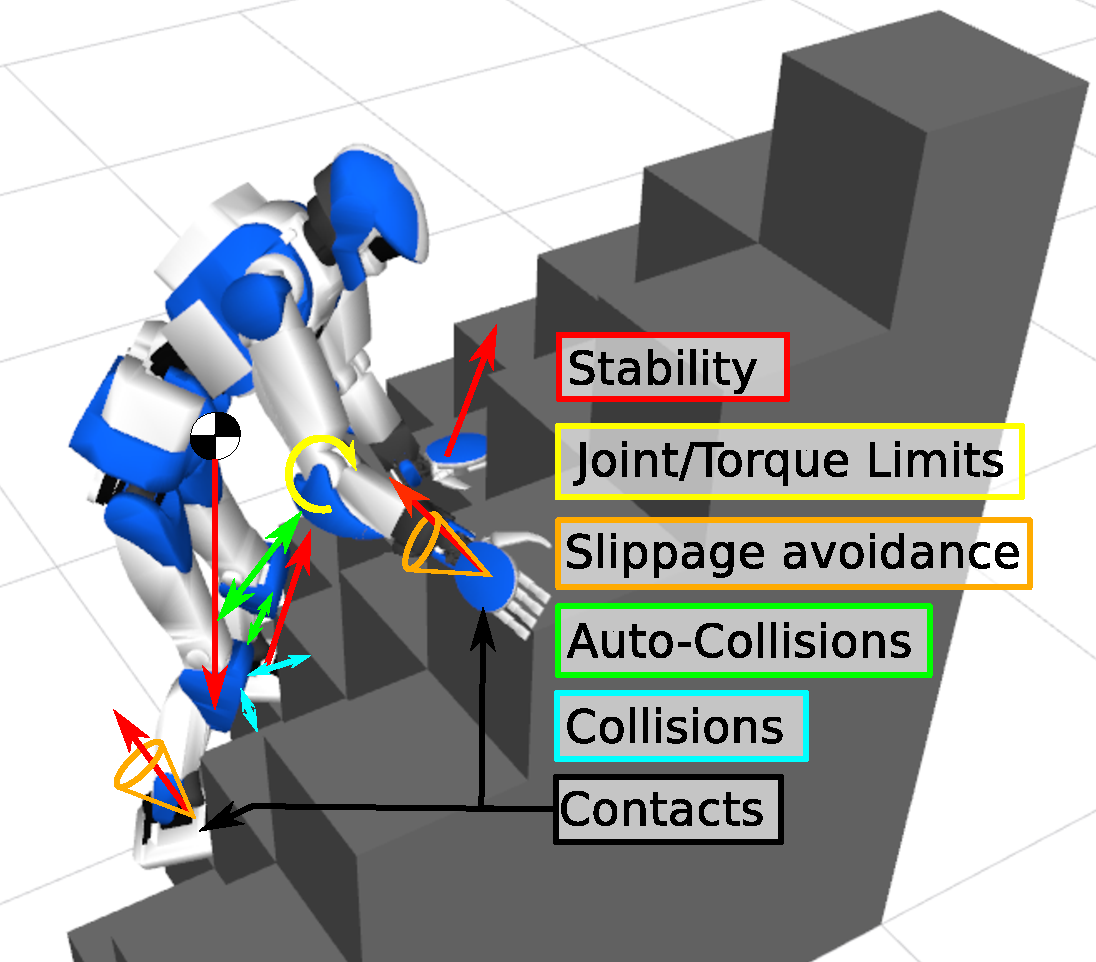
\includegraphics[width=0.7\textwidth]{PG.pdf}
  %\caption{HRP4 on a stack of cubes. The color of each box corresponds to the color of the item it depicts.}
%\label{fig:PG}
%\end{figure}


%%%%%%%%%%%%%%%%%%%%%%%%%%%%%%%%%%%%%%%%%%%%%%%%%%%%%%%%%%%%%%%%%%%%%%%
%                    SECTION PROBLEM FORMULATION                      %
%%%%%%%%%%%%%%%%%%%%%%%%%%%%%%%%%%%%%%%%%%%%%%%%%%%%%%%%%%%%%%%%%%%%%%%
%\section{Kinematics Formulation}
%\label{sec:kinematics_formulation}


\section{Forward Kinematics}
\label{sec:forward_kinematics}

%%%%%%%%%%%%%%%%%%%%%%%%%%%%%%%%%%%%%%%%%%%%%%%%%%%%%%%%%%%%%%%%%%%%%%%
%                   SUBSECTION FORWARD KINEMATICS                     %
%%%%%%%%%%%%%%%%%%%%%%%%%%%%%%%%%%%%%%%%%%%%%%%%%%%%%%%%%%%%%%%%%%%%%%%

In this section, we present a formulation of robotic systems that allows specifying most of the typical constraints encountered in robotics problems.

We consider a robotic system made of $n_B$ bodies and $n_J(=n_B+1)$ joints.
The global structure of the robot is described by an ordered graph called multibody graph.
The base body (World) has index $0$ and other bodies get different positive integer index.
We denote the body of index $i$, $B_i$.
$B_0$ refers to the World.
Each body $B_i$ has its reference frame $F_i$ attached to it.
$F_0$ denotes the World frame.
Bodies are linked together by joints that also are indexed by positive integers, we denote the joint of index $i$, $J_i$, and the body that comes after it is $B_i$.
Each joint defines the relation between its predecessor and successor bodies.
For joint $J_i$, they are respectively denoted $pred(i)$ and $succ(i)$, and $B_{pred(i)}$ is called the parent body of $B_{succ(i)}$.
We denote $\lambda(j)$ the index of the parent body of $B_j$.
The number of degrees of freedom of $J_i$ is denoted $dof^J_i$ and the number of degrees of freedom of the whole robot is denoted $dof$.
Figure~\ref{fig:mbg} illustrates this numbering system for a simple robot with 4 joints and 5 bodies (including the basis)

The geometric relations between bodies and joints are described through transformations between their reference frames.
We use transformations as described in the Spatial Vector Algebra chapter of `Rigid Body Dynamics Algorithm' by Roy Featherstone~\cite{featherstone:book:2007}.
Motion vectors (vectors describing motion quantities as positions, velocities and accelerations) and their force counterpart are defined in~\cite{featherstone:book:2007}.

For any 3D vector $v\in\mathbb{R}^3$, $\hat{v}$ denotes the $3\times 3$ skew-symmetric matrix such that $\hat{v}u = v\wedge u$.
Where $\wedge$ denotes the cross product operator.

Let A and B be Cartesian frames with origins O and P respectively.
Let $\mathbf{t}$ be the coordinate vector expressing $\overrightarrow{OP}$ in A.
And $\mathbf{R}$ be the rotation matrix that transforms 3D vectors from A to B coordinates.
The transformation from A to B for a motion vector is defined by:
\begin{equation}
  {}^B X_A =
  \begin{bmatrix}
    \mathbf{R} & \mathbf{0} \\
    -\mathbf{R}\hat{\mathbf{t}} & \mathbf{R} \\
  \end{bmatrix}
\end{equation}
Its inverse is:
\begin{equation}
  {{}^B X_A}^{-1} = {}^A X_B =
  \begin{bmatrix}
    \mathbf{R}^T & \mathbf{0} \\
    \hat{\mathbf{t}}\mathbf{R}^T & \mathbf{R}^T \\
  \end{bmatrix}
\end{equation}
The transformation from A to B for a force vector is defined by:
\begin{equation}
  {}^B X_A^* =
  \begin{bmatrix}
    \mathbf{R} & -\mathbf{R}\hat{\mathbf{t}} \\
    \mathbf{0} & \mathbf{R} \\
  \end{bmatrix}
\end{equation}
Its inverse is:
\begin{equation}
  {}^B X_A^{-*} = {}^A X_B^* =
  \begin{bmatrix}
    \mathbf{R}^T & \hat{\mathbf{t}}\mathbf{R}^T \\
    \mathbf{0} & \mathbf{R}^T \\
  \end{bmatrix}
\end{equation}

\begin{figure}
  \centering
  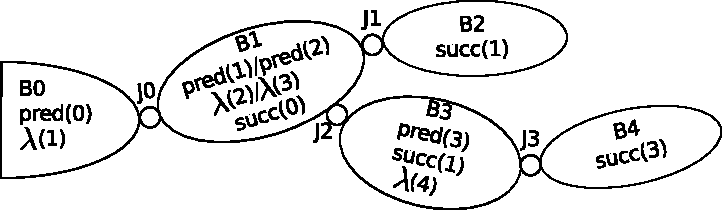
\includegraphics[width=0.7\textwidth]{mbg.pdf}
  \caption{MultiBody graph}
\label{fig:mbg}
\end{figure}

%Each joint $J_i$ is defined in the reference frame of its predecessor body by a static transformation $X^x_i = \{\mathbf{R}^x_i, \mathbf{t}^x_i\}$ from the base of the body to the base of the joint.
Each joint $J_i$ is defined by a static transformation $X^x_i = \{\mathbf{R}^x_i, \mathbf{t}^x_i\}$ between the reference frame of its predecessor body and its own reference frame.
Each joint $J_i$ is associated with a motion subspace which representation matrix is denoted $\mathbf{S}_i$.
Each column of $\mathbf{S}_i$ described a degree of freedom of $J_i$ its upper part for the rotations and lower for translations (see Section~\ref{sec:joints_formulations}).
\begin{equation}
  \mathbf{S}_i =
  \begin{bmatrix}
    S^R_{i,0} & \cdots &
    S^R_{i,j} & \cdots &
    S^R_{i,dof} \\
    S^t_{i,0} & \cdots &
    S^t_{i,j} & \cdots &
    S^t_{i,dof}
  \end{bmatrix}
\end{equation}

For a given joint configuration $q$, the transformation due to the joint $J_i$ current configuration from its reference frame to the reference frame of its successor body is denoted \\$X^J_i (q) = \{\mathbf{R}^J_i (q), \mathbf{t}^J_i (q)\}$.

The transformation between $B_{\lambda(i)}$ and $B_i$ is denoted $X^{PtS}_i (q) = \{\mathbf{R}^{PtS}_i, \mathbf{t}^{PtS}_i\}$ (PtS stands for `Parent to Son') can then be computed as:
\begin{equation}
  {X}^{PtS}_i (q) = {}^{i}X_{\lambda (i)} (q) = X^J_i (q) X^x_i
  \label{eq:PtS}
\end{equation}

Let $\kappa (i) =\{0, i_1, i_2 \ldots i\}$ be the list of indexes of successive joints going from $B_0$ to $B_i$.
It can easily be computed by adding iteratively the parent of the current body:

\begin{algorithm}
  \caption{Joint Path to $B_i$}
\label{alg:JP}
\begin{algorithmic}
  \State{$j \leftarrow i$, $\kappa(i)=[i]$}
  \While{$j \neq 0$}
  \State{$j \leftarrow \lambda(j)$}
  \State{$\kappa(i) \leftarrow [\kappa(i),\ j]$}
  \EndWhile{}
\end{algorithmic}
\end{algorithm}

The transformation from the World base to $B_i$ is denoted \\ ${}^i X_0 (q) = \{{}^i \mathbf{R}_0 (q), {}^i \mathbf{t}_0 (q)\}$.
The formula~\Eqref{eq:PtS} can be used iteratively on all bodies of the robot to obtain the expression of ${}^i X_0 (q)$.

We obtain the full expression of ${}^i X_0$ as:
\begin{equation}
  {}^i X_0 (q) = \prod_{j\in\kappa (i)}X^J_j (q) X^x_j = \prod_{j\in\kappa (i)}\ {}^j X_{\lambda (j)}
  = {}^i X_{\kappa (1)}\ ^{\kappa (1)}X_{\kappa (2)} \dots ^{\kappa (\text{end}-1)}X_{W}
\end{equation}

Which can be computed recursively by a Forward Kinematics algorithm:

\begin{algorithm}
  \caption{Forward Kinematics}
\label{alg:FK}
\begin{algorithmic}
  \For{$i = 0:n_J$}
  \If{$\lambda (i) \neq -1$} ${}^i X_0 = {}^i X_{\lambda (i)}\ ^{\lambda (i)}X_0$
  \Else$\ {}^i X_0 = X^{PtS}_i$
  \EndIf{}
  \EndFor{}
\end{algorithmic}
\end{algorithm}

In the following section, we provide some detailed description of how to compute $X_J (q)$ for a variety of useful joints.
Using the joint descriptions and the Forward Kinematics algorithm, we are able to explicit a relation between $q$ the joint parameters of the robot and the 3D position and orientation of  any geometric quantity defined in the reference frame of a body of the robot.
Given a transformation ${}^p X_i$ defined in the frame of $B_i$, its value in the world frame is given by ${}^p X_0 (q) = {}^p X_i\ {}^i X_0 (q)$



\section{Joints formulations}
\label{sec:joints_formulations}

%%%%%%%%%%%%%%%%%%%%%%%%%%%%%%%%%%%%%%%%%%%%%%%%%%%%%%%%%%%%%%%%%%%%%%%
%                   SUBSECTION JOINTS FORMULATIONS                    %
%%%%%%%%%%%%%%%%%%%%%%%%%%%%%%%%%%%%%%%%%%%%%%%%%%%%%%%%%%%%%%%%%%%%%%%

The entire geometry of our system is described by the list of static transformations $X^x_j$ and of joint transformations $X^J_j (q)$.
In this section, we explicit the descriptions and formulations of several useful joints.

Let us consider a joint $J$ that governs the transformation between two frames $F_1=\{O_1, x_1, y_1, z_1\}$ and $F_2=\{O_2, x_2, y_2, z_2\}$.
The most common type of joint encountered in robotics systems is the revolute joint, that allows a rotation around a fixed axis.
If $J$ is a revolute joint around the axis $(O_1,z_1)$ with parameter $q$, its motion subspace, rotation, and translation are as follows:

\begin{table} [ht]
\centering
\begin{tabular}{cccc}
  \toprule
  Joint type & $S$ & $Rotation$ & $translation$ \\
  \midrule
  Revolute $(O_1,z_1)$
  &
  $\begin{bmatrix}
    0 \\ 0 \\ 1 \\ 0 \\ 0 \\ 0
  \end{bmatrix}$
  &
  $\begin{bmatrix}
    1 & 0 & 0 \\
    0 & \cos (q) & \sin (q) \\
    0 & -\sin (q) & \cos (q) \\
  \end{bmatrix}$
  &
  ${\bf 0}_{3\times1}$
  \\
  \bottomrule
\end{tabular}
\end{table}

Similar formulas can be devised for rotations around any other axis, provided that $R$ describes the rotation of angle $q$ around that axis.

In the case of a prismatic joint, all rotations are blocked, and only one translation along a given axis is allowed.
A prismatic joint along $x_1$ is described by the following formulas:

\begin{table} [ht]
\centering
\begin{tabular}{cccc}
  \toprule
  Joint type & $S$ & $Rotation$ & $translation$ \\
  \midrule
  Prismatic $(x_1)$
  &
  $\begin{bmatrix}
    0 \\ 0 \\ 0 \\ 1 \\ 0 \\ 0
  \end{bmatrix}$
  &
  ${\bf 1}_{3\times3} $
  &
  $\begin{bmatrix}
    q \\ 0 \\ 0
  \end{bmatrix}$
  \\
  \bottomrule
\end{tabular}
\end{table}

Planar joints are also frequently used in robotics.
A planar joint describes a plan sliding on another plan, assuming that the normal to both plans is $z_1 = z_2$ this type of joint allows free rotation of $F_2$ around $z_1$ and translations along $x_1$ and $y_1$.
We denote $q = \{q_1, q_2, q_3\}$ the joint parameters, $q_1$ corresponding to the rotation and $q_2,\ q_3$ to the translations.
We get:

\begin{table} [ht]
\centering
\begin{tabular}{cccc}
  \toprule
  Joint type & $S$ & $Rotation$ & $translation$ \\
  \midrule
  Planar $(z_1)$
  &
  $\begin{bmatrix}
    0 & 0 & 0 \\ 0 & 0 & 0 \\ 1 & 0 & 0 \\ 0 & 1 & 0 \\ 0 & 0 & 1 \\ 0 & 0 & 0
  \end{bmatrix}$
  &
  $\begin{bmatrix}
    1 & 0 & 0 \\
    0 & \cos(q_1) & \sin(q_1) \\
    0 & -\sin(q_1) & \cos(q_1) \\
  \end{bmatrix}$
  &
  $\begin{bmatrix}
    \cos(q_1)q_2 - \sin(q_1)q_3 \\ \sin(q_1)q_2 + \cos(q_1)q_3 \\ 0
  \end{bmatrix}$
  \\
  \bottomrule
\end{tabular}
\end{table}

A spherical joint blocks all translations and allows all rotations.
This joint must be parameterized by a 3D rotation.
The space of 3D rotations $SO(3)$ can be represented in many different ways.
The simplest and most intuitive way to parameterize $SO(3)$ is to use Euler Angles.
It comes down to decomposing the 3D rotation into a succession of three 1D rotations around different axes.
For example, the roll, pitch, yaw is a succession of a rotation of $F_1$ around its $x$ axis, followed by a rotation of the resulting frame around its $y$ axis and a rotation of the resulting frame around its $z$ axis.
The rotation matrix for such a rotation is given by:
\begin{equation}
  {\bf R} =
  \begin{bmatrix}
    1 & 0 & 0 \\
    0 & \cos(q_3) & \sin(q_3) \\
    0 & -\sin(q_3) & \cos(q_3) \\
  \end{bmatrix}
  \cdot
  \begin{bmatrix}
    \cos(q_2) & 0 & -\sin(q_2) \\
    0 & 1 & 0 \\
    \sin(q_2) & 0 & \cos(q_2) \\
  \end{bmatrix}
  \cdot
  \begin{bmatrix}
    \cos(q_1) & \sin(q_1) & 0 \\
    -\sin(q_1) & \cos(q_1) & 0 \\
    0 & 0 & 1
  \end{bmatrix}
\end{equation}

Euler Angle formulations have the advantage to be simple and intuitive.
There are many other possible choices of axes to define a Euler Angle 3D rotation.
But they all suffer from singularities (the gimbal lock), which happens when two of the three rotation axes become aligned.
In such a configuration, the only rotations possible are one rotation around the two aligned axis and one rotation around the third axis.
Thus, one degree of freedom is lost.
Those singularities are prohibitive for the use of that type of formulation in a posture generation.
In~\cite{grassia1998}, Grassia states that any attempt to parameterize the entire set of 3D rotations by an open subset of Euclidean space(as do Euler angles) will suffer from gimbal lock.
Note that this singularity is only due to the user's choice of parameterization, it is not intrinsic to the manifold $SO(3)$.
%One can prove that there is no smooth mapping between $SO(3)$ and $\mathbb{R}^3$ that is free of singularities.
It is possible to parameterize $SO(3)$ without having to face singularities by parameterizing it over another non-Euclidean manifold.
The most common ones are the set of unit quaternion embedded in $\mathbb{R}^4$ and the set of rotation matrices embedded in $\mathbb{R}^{3\times 3}$.
%To avoid singularities, one must use a higher dimension parametrization, such as the most common $SO(3)$ representation in robotics that are the unit quaternions and the rotation matrices.
%The unit quaternions space is the subset of $\mathbb{R}^4$ where all elements have unit norm.
With the unit quaternion parameterization, a variable on $SO(3)$ is represented by 4 parameters $q = [q_w, q_x, q_y, q_z]$, and it is necessary to ensure that the quaternion is of norm 1, $\{q\in\mathbb{R}^4:||q||=1\}$.
Similarly, if a variable is parameterized by a rotation matrix, then the matrix $M$ representing it has 9 parameters and M must be orthogonal and have determinant 1: $\{M\in\mathbb{R}^{3\times 3}:M^T M = \mathbb{I}_3\  \&\ \det (M) = 1\}$.
Similar issues can be found with the parameterization of other non-Euclidean manifolds, like $S2$ for example.

A quaternion $q = [q_w, q_x, q_y, q_z]$ is a unit quaternion iff $q_w^2+q_x^2+q_y^2+q_z^2 = 1$.
It represents a rotation of angle $\theta$ around an axis ${\bf u}$ such that:
\begin{align}
  q_w &= \cos(\theta/2) \\
  q_x &= \sin(\theta/2)u_x \\
  q_y &= \sin(\theta/2)u_y \\
  q_z &= \sin(\theta/2)u_z \\
\end{align}
The rotation matrix associated with this quaternion is:
\begin{equation}
  {\bf R} = 2 \begin{bmatrix}
    \frac{1}{2} - {q_y}^2 - {q_z}^2 &	q_x q_y - q_z q_w &	q_x q_z + q_y q_w \\
    q_x q_y + q_z q_w	& \frac{1}{2} - {q_x}^2 - {q_z}^2 &	q_y q_z - q_x q_w \\
    q_x q_z - q_y q_w &	q_y q_z + q_x q_w	& \frac{1}{2} - {q_x}^2 - {q_y}^2 \\
  \end{bmatrix}
\end{equation}

That formulation does not suffer from singularities, but it requires to maintain 4 parameters for a 3D rotation.
And those 4 parameters must satisfy the unit norm constraint which in turn would become an additional constraint in the optimization formulation.
Given a parameter set $q = \{ q_w, q_x, q_y, q_z\}$, we get the following table.

\begin{table}[ht]
  \centering
  \begin{tabular}{cccc}
    \toprule
    Joint type & $S$ & $Rotation$ & $translation$ \\
    \midrule
    Spherical
    &
    $\begin{bmatrix}
      1 & 0 & 0 \\ 0 & 1 & 0 \\ 0 & 0 & 1 \\ 0 & 0 & 0 \\ 0 & 0 & 0 \\ 0 & 0 & 0
    \end{bmatrix}$
    &
    $2 \begin{bmatrix}
    \frac{1}{2} - {q_y}^2 - {q_z}^2 &	q_x q_y - q_z q_w &	q_x q_z + q_y q_w \\
    q_x q_y + q_z q_w	& \frac{1}{2} - {q_x}^2 - {q_z}^2 &	q_y q_z - q_x q_w \\
    q_x q_z - q_y q_w &	q_y q_z + q_x q_w	& \frac{1}{2} - {q_x}^2 - {q_y}^2 \\
    \end{bmatrix}$
    &
    $\begin{bmatrix}
      0 \\ 0 \\ 0
    \end{bmatrix}$
    \\
    \bottomrule
  \end{tabular}
\end{table}

Finally, a free joint allows free motion of its successor body with respect to its predecessor body.
It can be viewed as a combination of a spherical joint and 3 perpendicular prismatic joints.
Given a parameter set $q = \{ q_w, q_x, q_y, q_z, t_x, t_y, t_z\}$, we get the following table.

\begin{tabular}{cccc}
  \toprule
  Joint type & $S$ & $Rotation$ & $translation$ \\
  \midrule
  Spherical
  &
  $\mathbb{I}_6$
  &
  $2 \begin{bmatrix}
    \frac{1}{2} - {q_y}^2 - {q_z}^2 &	q_x q_y - q_z q_w &	q_x q_z + q_y q_w \\
    q_x q_y + q_z q_w	& \frac{1}{2} - {q_x}^2 - {q_z}^2 &	q_y q_z - q_x q_w \\
    q_x q_z - q_y q_w &	q_y q_z + q_x q_w	& \frac{1}{2} - {q_x}^2 - {q_y}^2 \\
  \end{bmatrix}$
  &
  ${\bf R}^{-1}\begin{bmatrix}
    t_x \\ t_y \\ t_z
  \end{bmatrix}$
  \\
  \bottomrule
\end{tabular}



\section{Jacobian computation}
\label{sec:jacobian_computation}

%%%%%%%%%%%%%%%%%%%%%%%%%%%%%%%%%%%%%%%%%%%%%%%%%%%%%%%%%%%%%%%%%%%%%%%
%                  SUBSECTION JACOBIAN COMPUTATION                    %
%%%%%%%%%%%%%%%%%%%%%%%%%%%%%%%%%%%%%%%%%%%%%%%%%%%%%%%%%%%%%%%%%%%%%%%

For the sake of solving our problem with a nonlinear optimization algorithm, it is useful to compute the derivatives of every function used as constraint or cost with respect to any variable of the problem.
The transformations ${}^i X_0$ are used in many functions, therefore, having an efficient algorithm to compute their derivatives and the derivatives of any transformation defined in $B_i$ is necessary.

Given a static transformation ${}^p X_i$ defined in body $B_i$.
Its expression in the world frame is ${}^p X_0 = {}^p X_i\ {}^i X_0$ and its expression in the frame of $B_j$ is ${}^p X_j = {}^p X_i\ {}^i X_0\ {{}^j X_i}^{-1}$.

We denote $\text{Jac}_i$ the Jacobian of body $i$, and $\text{Jac}_i(X)$ the jacobian of the frame defined by $X$ in the referential of body $i$.
$q_i$ is the part of $q$ that corresponds to the degrees of freedom of joint $J_i$.
We denote $\text{Jac}_i.\text{cols}(j)$ the columns of $\text{Jac}_i$ associated with joint $J_j$.
The jacobian of the frame defined by ${}^p X_i$ in $B_i$ with respect to $q_j$ is given by
\begin{equation}
\label{partial_jacobian}
  \text{Jac}_i({}^p X_i).\text{cols}(j) = {}^p X_j\ S_i
\end{equation}

The complete jacobian of a body $\text{Jac}_i$ is a $6\times \text{dof}$ matrix that can be computed by using the formula~\ref{partial_jacobian} on every index $j$ in $\kappa(i)$ and filling the rest of $\text{Jac}_i$ with zeros.

The algorithm that we use to compute $\text{Jac}_i({}{}^p X_i)$ writes as follows:

\begin{algorithm}
  \caption{Jacobian Computation}
\label{alg:jacobian_computation}
\begin{algorithmic}
  \State{$\text{Jac}_i({}^p X_i) = {\bf 0}_{6\times\text{dof}}$}
  \State{${}^p X_0 = {}^p X_i\ {({}^i X_0)}^{-1}$}
  \For{$j = 0:\text{size}(\kappa(i))$}
  \State{$k \leftarrow \kappa(j)$}
  \State{${}^p X_k = {}^p X_0\ {({}^k X_0)}^{-1}$}
  \State{$\text{Jac}_i({}^p X_i).\text{cols}(k) = {}^p X_k\ S_k$}
  \EndFor{}
\end{algorithmic}
\end{algorithm}

We write the jacobian of each body at its origin as follows:
\begin{equation}
  \mathbf{Jac}^0_i =
  \begin{bmatrix}
    \frac{\partial {}^i\mathbf{R}_0}{\partial q_0} & \cdots &
    \frac{\partial {}^i\mathbf{R}_0}{\partial q_j} & \cdots &
    \frac{\partial {}^i\mathbf{R}_0}{\partial q_{dof}} \\
    \frac{\partial {}^i\mathbf{t}_0}{\partial q_0} & \cdots &
    \frac{\partial {}^i\mathbf{t}_0}{\partial q_j} & \cdots &
    \frac{\partial {}^i\mathbf{t}_0}{\partial q_{dof}}
  \end{bmatrix}
=
  \begin{bmatrix}
    \omega_{i,0} & \cdots &
    \omega_{i,j} & \cdots &
    \omega_{i,dof} \\
    v_{i,0} & \cdots &
    v_{i,j} & \cdots &
    v_{i,dof}
  \end{bmatrix}
\end{equation}



%\section{Geometric constraints}
%\label{sec:geometric_constraints}

%%%%%%%%%%%%%%%%%%%%%%%%%%%%%%%%%%%%%%%%%%%%%%%%%%%%%%%%%%%%%%%%%%%%%%%
%          SECTION GEOMETRIC CONSTRAINTS                              %
%%%%%%%%%%%%%%%%%%%%%%%%%%%%%%%%%%%%%%%%%%%%%%%%%%%%%%%%%%%%%%%%%%%%%%%

\section{Joint Limits}
\label{sec:joint_limits}

%%%%%%%%%%%%%%%%%%%%%%%%%%%%%%%%%%%%%%%%%%%%%%%%%%%%%%%%%%%%%%%%%%%%%%%
%                      SUBSECTION JOINT LIMITS                        %
%%%%%%%%%%%%%%%%%%%%%%%%%%%%%%%%%%%%%%%%%%%%%%%%%%%%%%%%%%%%%%%%%%%%%%%

Most robotic joints have geometric limits which define the range of value that can be accessed by the joint variables.
The joint limits for 1D joints like revolute and prismatic joints are trivial to formulate: We denote $q^-$ and $q^+$ the lower and upper values accessible and add a boundary constraint to the optimization problem:
\begin{equation}
\label{eq:joint_limits}
  \boxed{q^- \leq q \leq q^+}
\end{equation}

Most joints are easy to limit because their variables are independent.
Limiting the movements of a spherical joint, and by extension, of a free joint, is more complicated.
In humanoid robotics, spherical joints can be used to model the shoulder or hip joint of the robot.
A common approach to limit shoulder joint, inspired from the biomechanics field, considers the spherical motion (or swing) and the axial motion (or twist) separately as shown in~\Figref{fig:ballAndSocket}.

\begin{figure}[htpb]
  \centering
  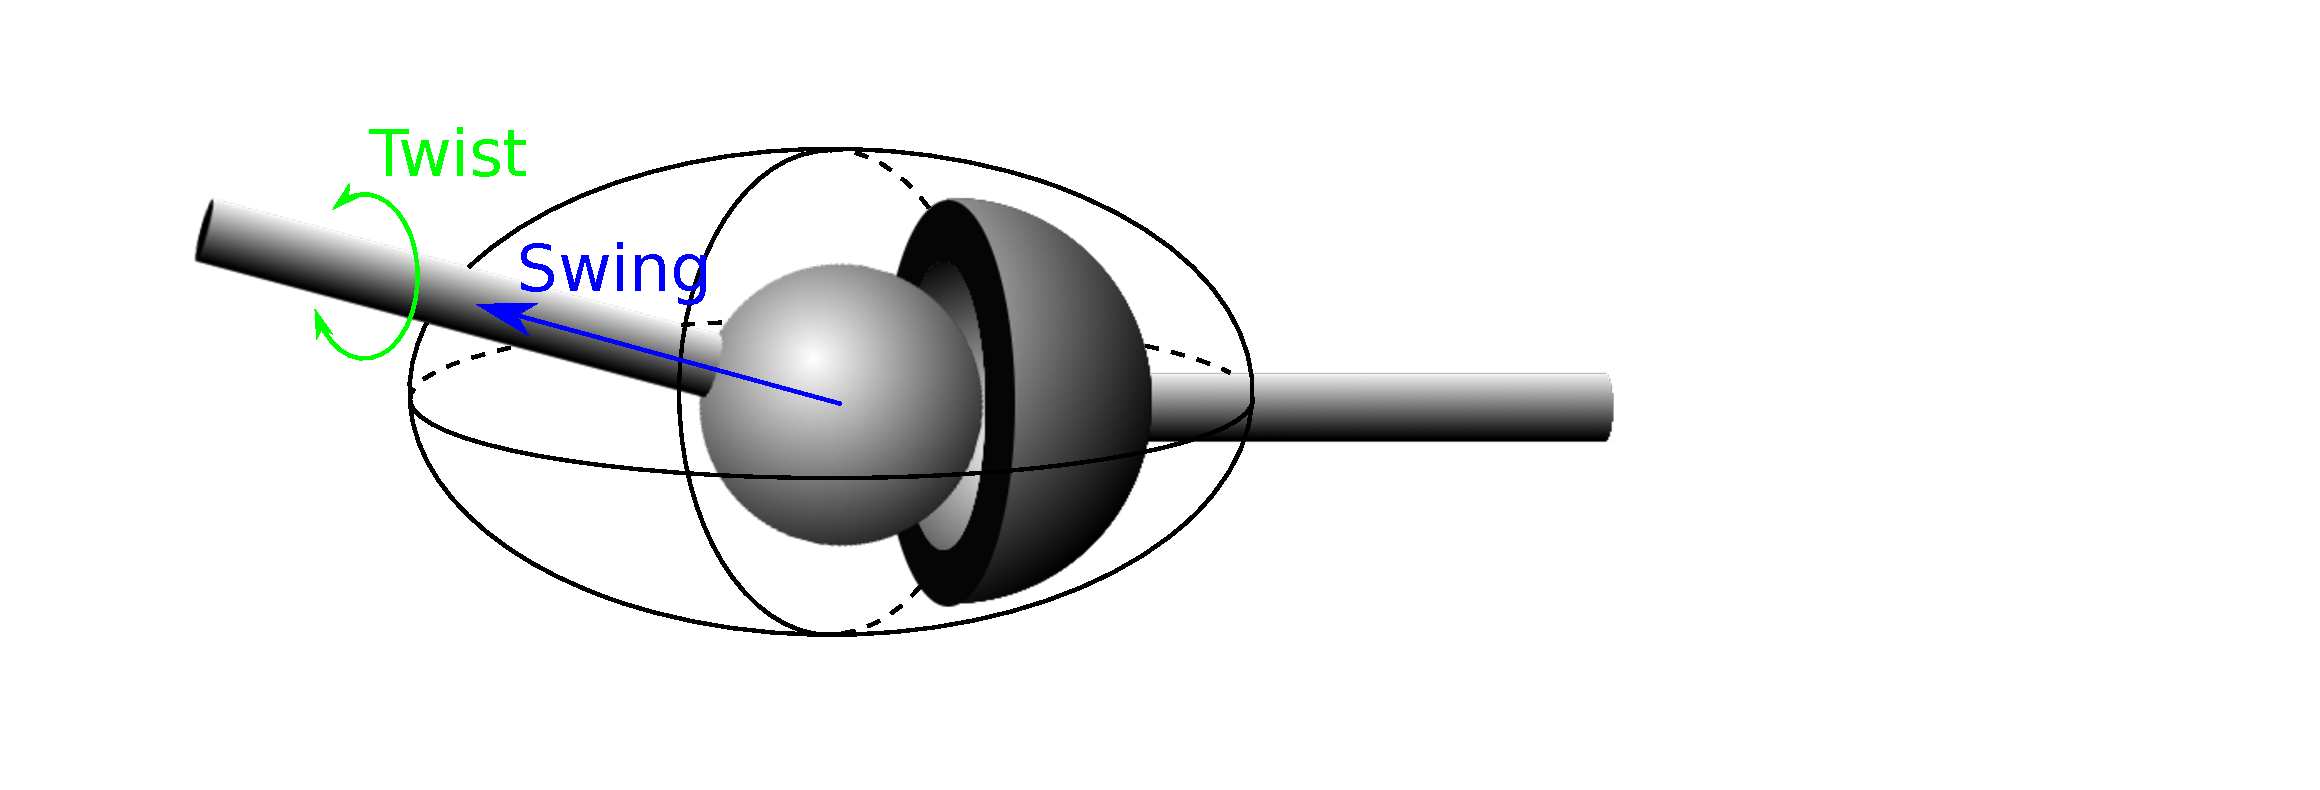
\includegraphics[width=0.7\linewidth]{ballAndSocket.pdf}
  \caption{Swing and Twist in ball and socket joint}
\label{fig:ballAndSocket}
\end{figure}

The spherical motion can be parameterized by a vector of the 3D unit sphere $S2$ and constrained to lay within a limit cone, the axial motion can be parameterized in $\mathbb{R}$ and limited by equation~\Eqref{eq:joint_limits}.
This type of formulation is presented in~\cite{baerlocher}.



\section{Contact constraints}
\label{sec:contact_constraints}

%%%%%%%%%%%%%%%%%%%%%%%%%%%%%%%%%%%%%%%%%%%%%%%%%%%%%%%%%%%%%%%%%%%%%%%
%                   SUBSECTION CONTACT CONSTRAINTS                    %
%%%%%%%%%%%%%%%%%%%%%%%%%%%%%%%%%%%%%%%%%%%%%%%%%%%%%%%%%%%%%%%%%%%%%%%

Humanoid robots evolve in their environment by making and breaking contacts with it.
A contact can be defined between 2 surfaces of different bodies of robots.
The most usual types of contact constraint encountered are the planar contact and the fixed contact.
A planar contact constraint is used when a planar surface of a robot is put in contact with a planar surface of the environment.
We denote $F_1 = \{O_1, \vec{x_1}, \vec{y_1}, \vec{z_1}\}$ a frame defined on $S_1$, the surface of the first body involved in the contact, such that the 3D point $O_1$ is on $S_1$ and the vector $\vec{z_1}$ is normal to $S_1$ and pointing toward the inside the body.
$F2 = \{O_2, \vec{x_2}, \vec{y_2}, \vec{z_2}\}$ is a frame on $S_2$, the surface of the second body involved, such that $O_2$ is on $S_2$ and the vector $\vec{z_2}$ is normal to $S_2$ and pointing away from the body.

Constraining $S_1$ and $S_2$ to be coplanar comes down to aligning $\vec{z_1}$ with $\vec{z_2}$ and to ensure that the projection of the distance between $O_1$ and $O_2$ along $\vec{z_1}$ is null.
Note that we avoid using the dot product of two vectors that are meant to be aligned e.g. $\vec{z_1}\cdot\vec{z_2} = 1$ because when that constraint is satisfied, its gradient is zero, which implies that in the optimization context it is unqualified.
That is why we prefer imposing orthogonality constraints.
This translates into adding the following set of constraints to our problem:

\begin{equation}
\label{eq:coplanarity}
\boxed{\left\{
  \begin{array}{l}
    \overrightarrow{O_1O_2} \cdot \vec{z_1} = 0\\
    \vec{x_1}\cdot\vec{z_2} = 0\\
    \vec{y_1}\cdot\vec{z_2} = 0\\
    \vec{z_1}\cdot\vec{z_2} \geq 0
  \end{array}
  \right.}
\end{equation}

This set of constraints leaves free the displacements of $F_2$ along $\vec{x_1}$ and $\vec{y_1}$ as well as its rotation around $\vec{z_1}$.
We call this a floating planar contact, the optimization algorithm will be able to choose the location of $F_2$ in the plane $\{O_1, \vec{x_1}, \vec{y_1}\}$.
This contact has 3 degrees of freedom.

\begin{figure}[htpb]
  \centering
  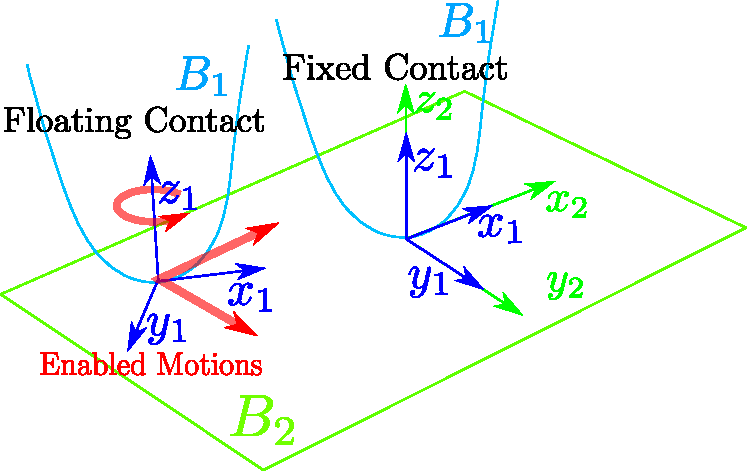
\includegraphics[width=0.8\linewidth]{contactConstraint.pdf}
  \caption{Floating and Fixed Contacts}
\label{fig:contactConstraint}
\end{figure}

If we constrain the location of $F_2$ in $\{O_1, \vec{x_1}, \vec{y_1}\}$ such that $O_1$ and $O_2$ are superimposed and $\vec{x_1}$, $\vec{y_1}$, $\vec{z_1}$ are aligned with respectively $\vec{x_2}$, $\vec{y_2}$, $\vec{z_2}$, we obtain a fixed contact with zero degrees of freedom.
This translates into adding the following set of constraints to our problem:

\begin{equation}
\label{eq:fixed_contact}
\boxed{\left\{
  \begin{array}{l}
    \overrightarrow{O_1O_2} = \vec{0}\\
    \vec{x_1}\cdot\vec{z_2} = 0\\
    \vec{y_1}\cdot\vec{z_2} = 0\\
    \vec{x_1}\cdot\vec{y_2} = 0\\
    \vec{z_1}\cdot\vec{z_2} \geq 0\\
    \vec{x_1}\cdot\vec{x_2} \geq 0\\
  \end{array}
  \right.}
\end{equation}

We illustrate those two types of contacts in~\Figref{fig:contactConstraint}



\section{Collision avoidance}
\label{sec:collision_avoidance}

%%%%%%%%%%%%%%%%%%%%%%%%%%%%%%%%%%%%%%%%%%%%%%%%%%%%%%%%%%%%%%%%%%%%%%%
%                   SUBSECTION COLLISION AVOIDANCE                    %
%%%%%%%%%%%%%%%%%%%%%%%%%%%%%%%%%%%%%%%%%%%%%%%%%%%%%%%%%%%%%%%%%%%%%%%

In order to avoid unwanted collisions between bodies of robots, for two bodies $B_1$ and $B_2$, we want to define a continuously differentiable function $d_{\{B_1, B_2\}}(q)$ that has the properties of a pseudo-distance:
\begin{itemize}
  \item $d_{\{B_1, B_2\}}(q) > 0$ when the bodies are not touching each other
  \item $d_{\{B_1, B_2\}}(q) = 0$ when the bodies are in collision without interpenetration
  \item $d_{\{B_1, B_2\}}(q) < 0$ when the bodies are in collision with interpenetration
\end{itemize}

Using the cartesian distance between the exact surfaces of $B_1$ and $B_2$ might result in a discontinuous gradient of $d_{\{B_1, B_2\}}$ if the surfaces of $B_1$ and $B_2$ are not strictly convex.
A conservative approach is to associate to each body, a strictly convex bounding volume and to compute the distance between those volumes.
\cite{escande:humanoids:2007} and~\cite{escande:itro:2014} proposes a method to generate a strictly convex Sphere-Torus-Patch Bounding Volumes (STP-BV) that guarantees the gradient continuity of the proximity distance.
The distance between the STP-BV of $B_1$ and $B_2$ computed by an enhanced GJK~\cite{gilbert-1988a} collision-detection algorithm is a continuously differentiable pseudo-distance.
Thus, we can use this function in our optimization algorithm to ensure that the distance between the bodies is greater than a safety distance $\epsilon_{12}$:

\begin{equation}
  \boxed{d_{\{B_1, B_2\}}(q) \geq \epsilon_{12}}
\end{equation}

This function can be used to avoid collisions between a robot and the environment as well as auto collisions between bodies of the same robot.
We denote $Coll$ the list of triplets $\{B_i, B_j, \epsilon_{ij}\}$ defining each collision that we want to avoid.

Then the set of constraints to add to our problem is:

\begin{equation}
  \boxed{\forall \{B_i, B_j, \epsilon_{ij}\} \in Coll,\ d_{\{B_i, B_j\}}(q) \geq \epsilon_{ij}}
\end{equation}

In many cases, it is possible to avoid the collision between two bodies of a robot by modifying the joint limits and reducing them to a span where the collision of interest cannot happen.
That approach is conservative and ad-hoc but can save some precious computation time.


%\section{Static constraints}
%\label{sec:static_constraints}

%%%%%%%%%%%%%%%%%%%%%%%%%%%%%%%%%%%%%%%%%%%%%%%%%%%%%%%%%%%%%%%%%%%%%%%
%                SECTION STATIC CONSTRAINTS                           %
%%%%%%%%%%%%%%%%%%%%%%%%%%%%%%%%%%%%%%%%%%%%%%%%%%%%%%%%%%%%%%%%%%%%%%%

\section{External Forces}
\label{sec:external_forces}

%%%%%%%%%%%%%%%%%%%%%%%%%%%%%%%%%%%%%%%%%%%%%%%%%%%%%%%%%%%%%%%%%%%%%%%
%                     SUBSECTION EXTERNAL FORCES                      %
%%%%%%%%%%%%%%%%%%%%%%%%%%%%%%%%%%%%%%%%%%%%%%%%%%%%%%%%%%%%%%%%%%%%%%%

For a robot to interact with the real world, its geometric description is not enough.
The robot is subject to forces applied on its bodies by the exterior world, which can be generated by contacts with the environment or with another actor (human, another robot, manipulated object\ldots), by the effect of physical forces like gravitation or magnetism, or by contacts between two bodies of the robot.
Our posture generator must take those `External forces' into account, to be able to estimate the stability of the robot and compute the internal torques generated in the joints.

An external force applied on a rigid body can also be called a wrench and is composed of a resultant part $f$ (sometimes called force) and a moment part (sometimes called couple).
Let $w$ be a wrench, $w|_F^O$ is the expression of $w$ calculated at the point $O$ expressed in the frame $F$.
We denote $\vec{f}$ the resultant part of w, and $\vec{f}|_F$ the expression of $\vec{f}$ in $F$.
$\vec{m}$ is the moment part of $w$ and $\vec{m}|_F^O$ the expression of $\vec{m}$ in $F$ calculated at the point $O$.

\begin{equation}
  w|_F^O = \left\{ \begin{array}{r}
    \vec{m}\\
    \vec{f}\\
  \end{array} \right\}^O_F
  = \left\{ \begin{array}{r}
    \vec{m}|_F^O\\
    \vec{f}|_F\\
  \end{array}\right\}
\end{equation}

The expression of the moment part on a different point $P$ is given by the following formula:

\begin{equation}
  \vec{m}|_F^P = \vec{m}|_F^O + \overrightarrow{PO} \wedge \vec{f}|_F
\end{equation}

The resultant part is invariant with respect to the point at which the wrench is calculated.

We drop the frame subscript when the choice of the frame does not matter and all quantities are computed in the same frame.



\section{Static stability}
\label{sec:static_stability}

%%%%%%%%%%%%%%%%%%%%%%%%%%%%%%%%%%%%%%%%%%%%%%%%%%%%%%%%%%%%%%%%%%%%%%%
%                    SUBSECTION STATIC STABILITY                      %
%%%%%%%%%%%%%%%%%%%%%%%%%%%%%%%%%%%%%%%%%%%%%%%%%%%%%%%%%%%%%%%%%%%%%%%

We denote $g$ the acceleration of gravity on earth $g = 9.81 m.s^{-2}$.
The wrench associated with the action of gravity on a body of mass $M$ which center of mass is denoted $G$ with $\vec{z}$ the upward vertical vector in the world frame $F_0$ is:
\begin{equation}
  w_g|^G_{F_0} = \left\{ \begin{array}{r}
     \vec{0} \\
     -Mg\vec{z} \\
 \end{array}\right\}^G_{F_0}
\end{equation}

A solid is statically stable if it satisfies the Euler-Newton Equation.
We consider a robot on which $m$ external wrench $w_i = \left\{ \begin{array}{r}
    \vec{m_i}\\
    \vec{f_i}\\
\end{array} \right\}^{P_i}$ are applied.
We denote $P$ the application point at which the equation and all its terms are calculated:
\begin{equation}
  \sum\limits_i w_i|^P + w_g|^P = 0
\end{equation}
which is equivalent to:
\begin{equation}
\left\{
\begin{array}{r}
  \sum\limits_i \vec{m_i}|^P + \overrightarrow{GP}\wedge Mg\vec{z} = 0 \\
  \sum\limits_i \vec{f_i} - Mg\vec{z} = 0 \\
\end{array}
\right.
\end{equation}

This equation can be simplified by applying it at the center of mass of the body as:
\begin{equation}
  \left\{
  \begin{array}{r}
    \sum\limits_i \vec{m_i}|^G = 0 \\
    \sum\limits_i \vec{f_i} - Mg\vec{z} = 0 \\
  \end{array}
  \right.
\label{eq:stability}
\end{equation}

Satisfying equation~\Eqref{eq:stability} ensures the stability of a rigid body.
If the robot's actuators are powerful enough to maintain its posture under any external perturbation, namely, when they can generate infinite or at least large enough torques, then the robot can be approximated as a rigid body and satisfying equation~\Eqref{eq:stability} is enough to ensure its stability.
%In some cases, an articulated robot is considered as a rigid body and this equation alone can be used to ensure its stability.
%It is only valid if the robot can generate infinite torques in its articulations, or at least if we have some guarantee that the robot is able to generate large enough torques.
Otherwise, it is necessary to verify that the robot's actuators can generate large enough torques to maintain that posture.
The details of torque computation are discussed in Section~\ref{sec:torque_limits}

Equation~\Eqref{eq:stability} can be used in an optimization problem.
We consider that each wrench $w_i$ applied on the system is defined by the position of its application point $P_i$ and the values $m_i$ and $f_i$ that represent the moment and resultant of $w_i$ at $P_i$.
$P_i$ depends on $q$ the joint parameter of the robot.
$m_i$ and $f_i$ are new variables that need to be added to the problem.
In summary, $w_i$ depends on $q$, $m_i$ and $f_i$.
We denote $f$ the concatenation of all the variables $m_i$ and $f_i$.

\begin{equation}
  \boxed{s(q,f) = \left\{
  \begin{array}{r}
    \sum\limits_i \vec{m_i} + \overrightarrow{P_i G}\wedge \vec{f_i} \\
    \sum\limits_i \vec{f_i} - Mg\vec{z} \\
  \end{array}
  \right\}
  = 0}
\end{equation}

The optimization problem~\Eqref{eq:optim_form_PG} becomes (we denote m the dimension of the force variables):

\begin{equation}
\label{eq:optim_form_PG_with_stab}
  \left\{
  \begin{array}{l}
    \min\limits_{q\in\mathcal{C}, f\in \mathbb{R}^m}{f(q)}\\
    \text{ s.t. }
    \left\{
    \begin{array}{l}
      s(q,f) = 0\\
      c_i(q) = 0,\ \forall i\in{E}\\
      c_i(q) \geq 0,\ \forall i\in{I}\\
    \end{array}
    \right.
  \end{array}
  \right.
\end{equation}

The derivation of the static stability constraint is straightforward.
All the terms of equation~\Eqref{eq:stability} are components of wrenches.
A wrench is completely defined by the frame in which it is expressed and its values of resultant and moment in that frame.
Deriving the stability condition comes down to deriving each term w.r.t its components values and w.r.t the transformation of its frame.

\begin{equation}
\left\{
\begin{array}{r}
  \partial\left(\sum\limits_i m_i|^G\right) = \sum\limits_i \partial(m_i|^G) \\
  \partial\left(\sum\limits_i f_i\right) = \sum\limits_i \partial(f_i) \\
\end{array}
\right.
\label{eq:derivation_stability}
\end{equation}

We will explicit a method to automatically compute those derivatives in a further chapter.



\section{Center of mass projection}
\label{sec:center_of_mass_projection}

%%%%%%%%%%%%%%%%%%%%%%%%%%%%%%%%%%%%%%%%%%%%%%%%%%%%%%%%%%%%%%%%%%%%%%%
%                SUBSECTION CENTER OF MASS PROJECTION                 %
%%%%%%%%%%%%%%%%%%%%%%%%%%%%%%%%%%%%%%%%%%%%%%%%%%%%%%%%%%%%%%%%%%%%%%%

When all the wrenches applied to the body are due to unilateral punctual contacts on the same horizontal plane $H = \{O, \vec{x}, \vec{y}\}$, the stability criterion~\Eqref{eq:stability} can be simplified.
The wrench $w_i$ generated by a unilateral punctual contact is a pure force resultant, its moment part is zero on the contact point.

\begin{equation*}
    \left. w_i \right|^{P_i} =
    \left\{
      \begin{array}{r}
      \vec{0}\\
      \vec{f_i}\\
  \end{array} \right\}^{P_i}
\end{equation*}

Equation~\Eqref{eq:stability} becomes:

\begin{equation}
\left\{
\begin{array}{r}
  \sum\limits_i \overrightarrow{OP_i}\wedge \vec{f_i} - \overrightarrow{OG} \wedge Mg\vec{z} = 0 \\
  \sum\limits_i \vec{f_i} - Mg\vec{z} = 0 \\
\end{array}
\right.
\end{equation}

We can write $\overrightarrow{OG} = \overrightarrow{OG_p} + z_G\vec{z}$ with $G_P$ the projection of $G$ on $H$. Replacing in the moment equation gives:

\begin{equation}
  \sum\limits_i \overrightarrow{OP_i}\wedge \vec{f_i} - \sum\limits_i\overrightarrow{OG_P} \wedge \vec{f_i} = 0
\label{eq:projCoM}
\end{equation}

With $f_i = f_i^x\vec{x} + f_i^y\vec{y} + f_i^z\vec{z}$, $G$ and $P_i$ can be written as $\overrightarrow{OG_P} = G_x \vec{x} + G_y\vec{y}$ and $\overrightarrow{OP_i} = P_{ix} \vec{x} + P_{iy} \vec{y}$. The two first lines of equation~\Eqref{eq:projCoM} give:

\begin{align}
\sum\limits_i \left\{\begin{array}{r} P_{iy}f_i^z\\-P_{ix}f_i^z\end{array}\right\}
= \left\{\begin{array}{r} G_{y}\\-G_{x}\end{array}\right\} \sum\limits_i f_i^z\\
  \overrightarrow{OG_P} = \frac{\sum\limits_i \overrightarrow{OP_i} f_i^z}{\sum\limits_i f_i^z}
\end{align}

Since all the contacts are unilateral, all the $f_i^z$ are positive.
For any set of $f_i^z\geq0$, $G_P$ is a barycenter with positive coefficients of the $P_i$.
Any point $G_P$ that is included in the convex hull of all the $P_i$ is a solution.

Thus, we have the property: a rigid body that has all its contacts with the environment being punctual, unilateral and all lying on the same horizontal plane $H$ is stable if and only if the projection of its center of mass on $H$ is inside the convex hull of all its contact points.



\section{Torque limits}
\label{sec:torque_limits}

%%%%%%%%%%%%%%%%%%%%%%%%%%%%%%%%%%%%%%%%%%%%%%%%%%%%%%%%%%%%%%%%%%%%%%%
%                      SUBSECTION TORQUE LIMITS                       %
%%%%%%%%%%%%%%%%%%%%%%%%%%%%%%%%%%%%%%%%%%%%%%%%%%%%%%%%%%%%%%%%%%%%%%%

In general, satisfying equation~\Eqref{eq:stability} is not enough to ensure that a robot can be statically stable.
The joint torques that are required to hold the posture must be within the physical capabilities of the robot, namely, its torque limits.
We denote $\tau_i^-$ and $\tau_i^+$ the minimal and maximal torques that can be generated by the robot's actuators on joint $J_i$.
In some cases, the torque limits can depend on the joint parameters $\tau_i^-(q)$ and $\tau_i^+(q)$.
For example, it is the case with the Atlas robot that is hydraulically actuated.

Featherstone~\cite{featherstone:book:2007} proposes a recursive algorithm to compute the torques, accelerations, and velocities generated in a multi-articulated system by a set of external forces called the Inverse Dynamics Algorithm.
For the purpose of generating statically stable postures, the velocities and accelerations are useless.
Thus, we devise a specialized algorithm to fit our needs and call it the Inverse Static Algorithm.

We denote $a_g$ the gravity acceleration vector with $\vec{a_c}$ its rotation part and $\vec{a_f}$ its translation part:
\begin{equation}
  a_g = \left\{ \begin{array}{r}
    \vec{a_c} \\
    \vec{a_f} \\
  \end{array} \right\}
  = \left\{ \begin{array}{r}
    \vec{0} \\
    g\vec{z}\\
  \end{array} \right\}
\end{equation}

The algorithm first computes the generalized forces $f^G_i$ applied to each body.
It is the sum of the action of gravity and of the external forces applied on a body calculated at the origin of the world frame, expressed in the world frame.
Then, the generalized forces are used to compute the torques.
We denote $\mathbf{I}_i$ the inertia matrix of body $i$.

\begin{algorithm}
  \caption{Inverse Static Algorithm}
\label{alg:IS}
\begin{algorithmic}
  \For{$i = 0:n_B$}
  \State$f^G_i = \mathbf{I}_i {}^i\mathbf{X}_0 a_g - {{}^i\mathbf{X}_0}^*f_i^{ext}$
  \EndFor{}
  \For{$i = n_J-1:0$}
  \State$\tau_i = {f^G_i}^T S_i$
  \If{$pred(i) \neq -1$}
  \State$f^G_{pred(i)} += {\mathbf{X}^{PtS}_i(q)}^{-*} f^G_i$
  \EndIf{}
  \EndFor{}
\end{algorithmic}
\end{algorithm}

We can write the torques as a function of the joint parameters and the external forces $\tau(q,f)$.
The torque limit constraint writes as:
\begin{equation}
  \boxed{\tau^- \leq \tau(q,f) \leq \tau^+}
\end{equation}

We will detail the derivation of this constraint in Section~\ref{sec:torque_derivation}.


\section{Contact Forces and Friction Cones}
\label{sec:contact_forces_and_friction_cones}

%%%%%%%%%%%%%%%%%%%%%%%%%%%%%%%%%%%%%%%%%%%%%%%%%%%%%%%%%%%%%%%%%%%%%%%
%            SUBSECTION CONTACT FORCES AND FRICTION CONES             %
%%%%%%%%%%%%%%%%%%%%%%%%%%%%%%%%%%%%%%%%%%%%%%%%%%%%%%%%%%%%%%%%%%%%%%%

%Here we use the same frames and notations as introduced in Section~\ref{sec:contact_constraints}.

The contacts involved in a posture generation problem can be separated into two types: Geometric Contacts and Stability Contacts.

The Geometric Contact is a contact where the position of contact is reached, but that contact does not support any contact forces (this is a necessary step to generate a sequence of quasi-static transitions).
Physically, that correspond to the transition state between a configuration without contact and a configuration with contact on which forces are applied.
We defined the Geometric Contacts in Section~\ref{sec:contact_constraints}.
The Stability Contact is a Geometric Contact that bears interaction forces.

%In planning, contacts are added or removed one by one between successive postures.
%In order to add or remove a stability contact, it is necessary to go through a geometric contact (that guarantees the continuity on contact forces).
%First a geometric contact configuration is found, then on the next posture, that geometric contact is fixed ond forces are added on it, it becomes a stability contact.
%Similarly, to remove a stability contact, we first look for a posture with a fixed geometric contact in place of the stability contact to remove.
%And on the next posture, the contact can be removed.

We denote $w_{1\rightarrow 2}$ the force applied by body $B_1$ on body $B_2$.
Then the force applied by $B_2$ on $B_1$ is $w_{2\rightarrow 1} = -w_{1\rightarrow 2}$.
%These interaction forces must be taken into account in the stability and torque computations of each robot involved in the contact.

The interaction force resulting from a punctual contact (see~\Figref{fig:frictionCone}) on a point $P$ can be modeled as a pure force resultant along the $z_1$ direction $\vec{f_n} = f_z \vec{z_1}$ and the tangential efforts due to the friction in that contact can be modeled as $\vec{f_t} = f_x \vec{x_1} + f_y \vec{y_1}$.
%A punctual contact cannot carry moments on its contact point.

\begin{equation}
\label{eq:punctual_force}
\left. w_{2\rightarrow 1}\right|^P = \left\{
  \begin{array}{l}
    \vec{0} \\
    \overrightarrow{f_{2\rightarrow 1}} = \vec{f_t} + \vec{f_n} \\
  \end{array}
  \right\}^P
\end{equation}

\begin{figure}[htpb]
  \centering
  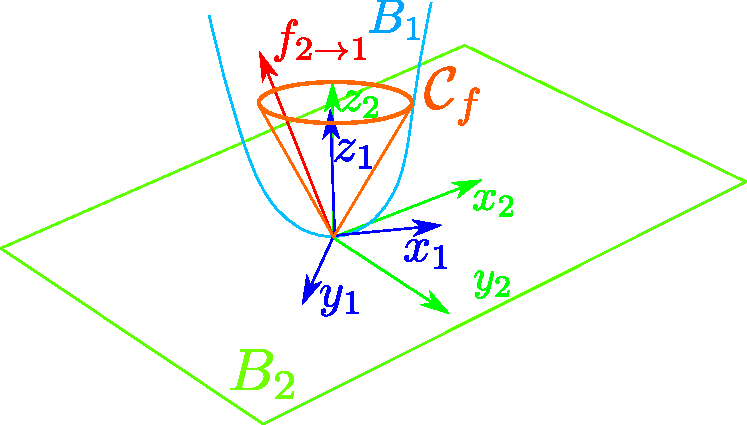
\includegraphics[width=0.6\linewidth]{frictionCone.pdf}
  \caption{Punctual unilateral stability contact with friction}
\label{fig:frictionCone}
\end{figure}

This formulation of the interaction force defines a bilateral contact, in the sense that the force can be in any direction, $B_1$ can push as well as pull on $B_2$.

To model a unilateral contact, we must constrain the normal component of $f_{2\rightarrow 1}$ to be oriented toward the inside of $B_1$.
This means that only pushing actions can be generated, not pulling actions.
This translates into:
\begin{equation}
  \overrightarrow{f_{2\rightarrow 1}}\cdot \vec{z_1} = f_z \geq 0
\end{equation}

Furthermore, to avoid slippage, the Coulomb friction law must be respected for each contact force $\vec{f}$.
%This law states that the contact force resultant must lay inside a friction cone of angle $\mu$, the friction coefficient.
Which translates into the following equation, with $\vec{f_n}$ and $f_t$, respectively the normal and tangential parts of $\vec{f}$ and $\mu$, the friction coefficient:

\begin{equation}
  \mu\|\vec{f_n}\| \geq \|\vec{f_t}\|
\end{equation}

Given the decomposition of $f_{2\rightarrow 1}$ in $F_1$, $f_{2\rightarrow 1} = f_x \vec{x_1} + f_y \vec{y_1} + f_z \vec{z_1}$, for any punctual contact in a posture generation problem, we can add the following set of constraint to our optimization problem:

\begin{equation}
  \label{eq:unilateralContact}
  \left\{
  \begin{array}{l}
    f_z \geq 0 \\
    \mu^2 f_z^2 - f_x^2 +f_y^2 \geq 0
  \end{array}
  \right.
\end{equation}

When it comes to planar contacts on surface $S$ with $\vec{n}$ the outbound normal to $S$, the interaction force can have components of forces and moments in all directions.
The forces components intrinsic to the planar contact model are a resultant part aligned with $\vec{n}$ $\vec{f_n} = f_z \vec{z_1}$ and a moment part tangential to $S$: $\vec{m_t} = m_x \vec{x_1} + m_y \vec{y_1}$.
The forces due to friction are a tangential friction resultant part $\vec{f_t} = f_x \vec{x_1} + f_y \vec{y_1}$ and a normal friction moment $\vec{m_n} = m_z \vec{z_1}$.

This type of force can be modeled by a set of unilateral punctual efforts applied on each vertex of a polygon describing the contact area.
And ensuring that each of them lay in their respective friction cone, thus satisfying the equation~\Eqref{eq:unilateralContact}.
As depicted in~\Figref{fig:planarContact}

\begin{figure}[htpb]
  \centering
  \setlength{\fboxsep}{0pt}%
  \setlength{\fboxrule}{1pt}%
  \fbox{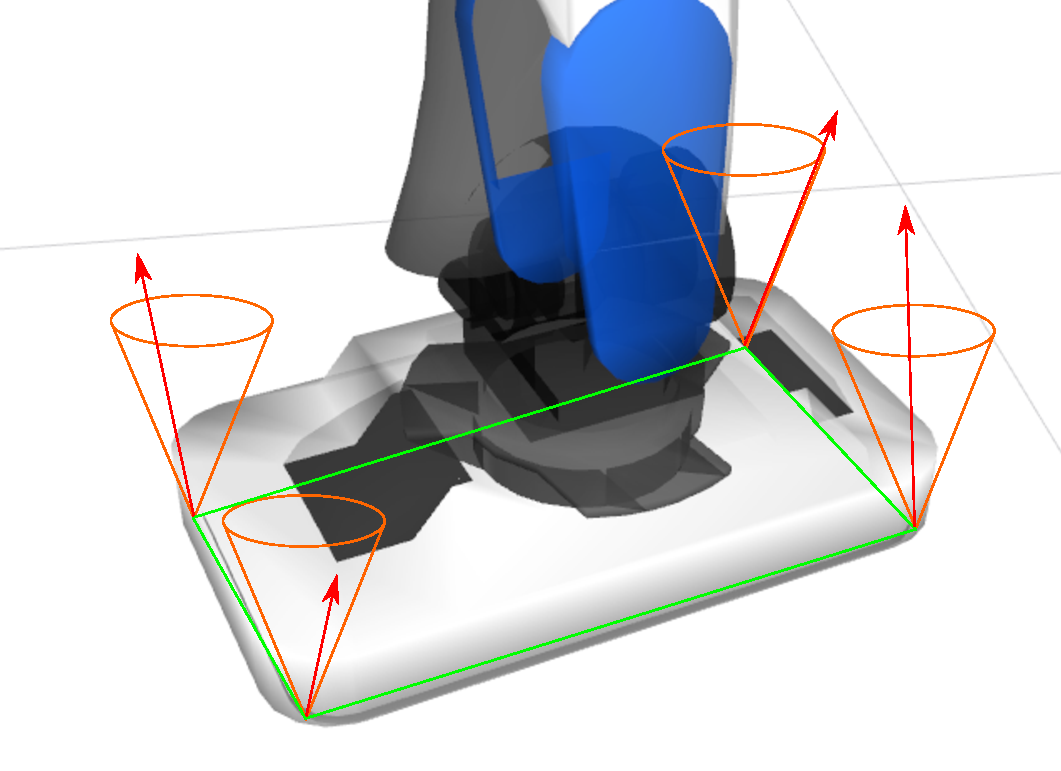
\includegraphics[width=0.6\linewidth]{planarContact.pdf}}
  \caption{Modelization of a Planar Contact between the foot on HRP4 and the ground}
\label{fig:planarContact}
\end{figure}



\section{Cost Functions}
\label{sec:cost_functions}

%%%%%%%%%%%%%%%%%%%%%%%%%%%%%%%%%%%%%%%%%%%%%%%%%%%%%%%%%%%%%%%%%%%%%%%
%                       SECTION COST FUNCTIONS                        %
%%%%%%%%%%%%%%%%%%%%%%%%%%%%%%%%%%%%%%%%%%%%%%%%%%%%%%%%%%%%%%%%%%%%%%%

In addition to constraints, it is often useful to add a cost function to our optimization problem.
The submanifold of feasible configurations $\mathcal{C}_F$ can contain an infinity of solutions and even some continuous solution areas in which all points are solutions.
The cost function helps to choose the `best' candidate solution.
Various types of cost functions can be chosen, for example, we can minimize the distance to a reference posture $q_R$:

\begin{equation*}
  f_\text{posture}(q) = {\|q-q_R\|}^2
\end{equation*}

The effect of that type of cost function is illustrated in~\Figref{fig:cost}.
On both images, the HRP-2 Kai robot is stable, respects its joints and torques limits.
The only difference is that the right one minimizes the distance to a reference posture (standing straight with bent knees) while the left result does not use a cost function.

\begin{figure}[htpb]
  \centering
  \setlength{\fboxsep}{0pt}%
  \setlength{\fboxrule}{1pt}%
  \fbox{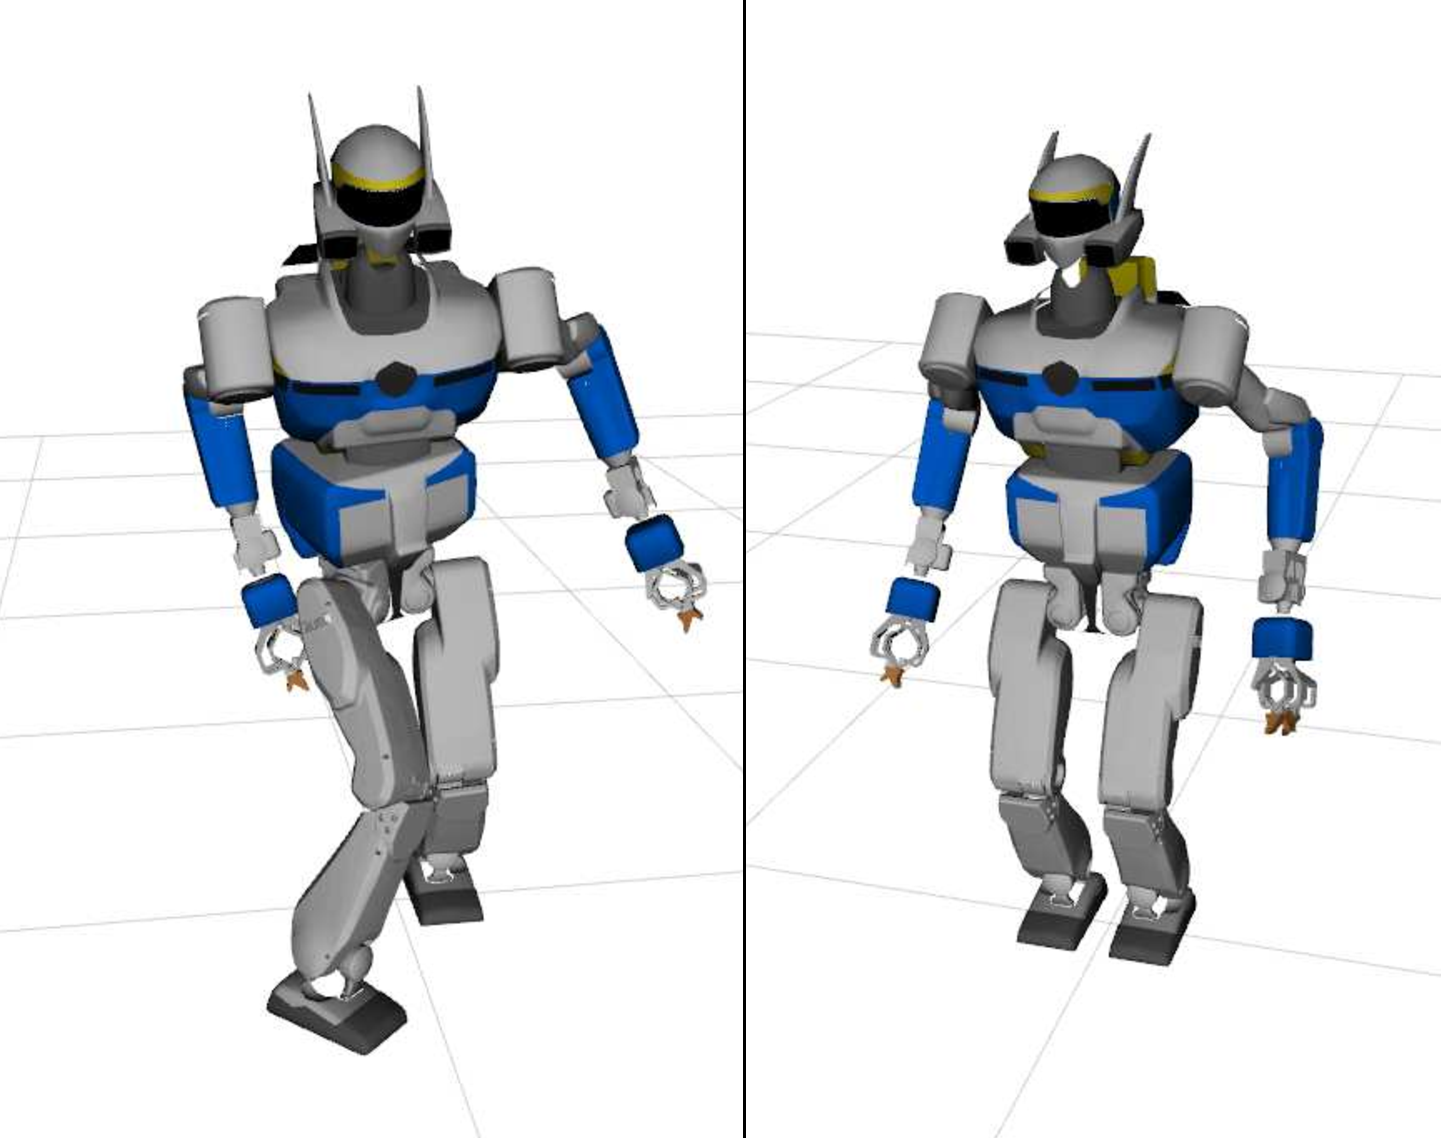
\includegraphics[width=0.5\linewidth]{cost.pdf}}
  \caption{Effect of cost function. Left: no cost function. Right: Distance to posture}
\label{fig:cost}
\end{figure}

We can also want to minimize the sum of norms of contact forces:
\begin{equation*}
  f_\text{forces}(f) = \sum\limits_i {\|f_i(f)\|}^2
\end{equation*}
or the torques in the robot's joints:
\begin{equation*}
  f_\text{torques}(q,f) = \sum\limits_i {\|\tau_i(q,f)\|}^2
\end{equation*}
Some more custom cost functions can also be considered, for example, we may want a point $P_i$ on body $B_i$ with to be as far as possible in a direction $\vec{d}$
\begin{equation*}
  f_\text{point} (q) = -{\overrightarrow{O_0 P_i}}\cdot{\vec{d}}
\end{equation*}

Any positively weighted combination of cost function can be used, in which case it is important to choose the weights $p_i$ carefully to scale all the costs so that they all can influence the result and none is completely dominated by another.
\begin{equation}
  f_\text{cost}(q,f) = \sum\limits_i{p_i f_i(q,f)} = p_0 f_\text{posture}(q) + p_1 f_\text{forces}(f) + p_2 f_\text{torques}(q,f) + \cdots
\end{equation}



\section{Conclusion}
\label{sec:Ch1_Conclusion}

%%%%%%%%%%%%%%%%%%%%%%%%%%%%%%%%%%%%%%%%%%%%%%%%%%%%%%%%%%%%%%%%%%%%%%%
%                         SECTION CONCLUSION                          %
%%%%%%%%%%%%%%%%%%%%%%%%%%%%%%%%%%%%%%%%%%%%%%%%%%%%%%%%%%%%%%%%%%%%%%%

In this section, we have seen how to formulate a robotics problem with several different tasks and objectives as an optimization problem.

We denote $\mathcal{T}_i$ the additional tasks added to the problem, which is described by the set of equations $g_i(q,f) = 0$ and inequations $h_i(q,f) \geq 0$.
The contact tasks are included in those and the equations describing them must encompass the geometric contact constraint equation like~\Eqref{eq:coplanarity} as well as the unilaterality and friction equations~\Eqref{eq:unilateralContact} in the case of a unilateral contact.

A typical robotics problem can be written as a combination of all those costs and constraints:
\begin{align}
\minimize_{q, f} & \quad f_\text{cost}(q,f) \nonumber\\
\text{s.t.}&
\left\{
\begin{array}{lr}
q^- \le q \le q^+\\
s(q,f) = 0 \\
\tau^- \le \tau(f,q) \le \tau^+\\
\forall \{B_i, B_j, \epsilon_{ij}\} \in Coll,\ d_{\{B_i, B_j\}}(q) > \epsilon_{ij}\\
g_i(q,f) = 0\ \ \forall\mathcal{T}_i,\\
h_i(q,f) \geq 0\ \ \forall\mathcal{T}_i.
\end{array}\right.
\label{eq:PG}
\end{align}

In the next chapter, we present an extension to the contact constraint formulation that allows generating non-inclusive contacts, an algorithm to compute the exact derivatives of the torques in robot's joints, and our endeavor to apply a different optimization approach to solving posture generation problems.
